\documentclass[12pt]{exam}
\usepackage{graphicx} % Required for inserting images
\usepackage{amssymb}
\usepackage{amsmath}
\usepackage{optidef}
\usepackage{listings}
\usepackage{xcolor} % for custom colors

\lstset{
  language=Python,
  basicstyle=\ttfamily\small,
  keywordstyle=\color{blue},
  stringstyle=\color{red},
  commentstyle=\color{gray},
  showstringspaces=false,
  frame=single,
  breaklines=true
}
\title{15.051 Mathematical programming, HW1}
\author{Erich Trieschman}
\date{2025.09.18}
\begin{document}
\maketitle

\begin{questions}
    \question \textbf{Optimal production schedule}
    
    Setup: 
    \begin{align*}
        \textbf{Constants}\\
        d \in \mathbb{R}^{12} \tag{product units to deliver}\\
        c_1 \in \mathbb{R} \tag{monthly cost of storing product}\\
        c_2 \in \mathbb{R} \tag{monthly cost of production change}\\
        \textbf{Variables}\\
        x \in \mathbb{R}^{12}  \tag{monthly production}\\
        \Delta x \in \mathbb{R}^{12} \tag{change in monthly production}\\
        I \in \mathbb{R}^{12}\tag{monthly inventory}\\
        \textbf{Objective}\\
        \sum_{i=1}^{11} c_1 I_i \tag{inventory cost; none in final month}\\
        \sum_{i=2}^{12} c_2 |\Delta x_i| \tag{production change cost}\\
        \textbf{Constraints}\\
        I_1 = 0, \; I \geq 0 \tag{no starting inventory; never negative inventory}\\
        x_1 \geq d_1, \; I_i + x_i \geq d_i \tag{always meet demand}\\
        \Delta x_i = x_i - x_{i-1}, \; i=2, \dots, 12 \tag{define change in production}\\
        I_i = I_{i-1} + x_i - d_i, \; i=2, \dots, 12 \tag{define inventory}\\
    \end{align*}
    Initial formulation (not LP):
    \begin{align*}
      \min_{I, x, \Delta x} \quad & \sum_{i=1}^{11} c_1 I_i + \sum_{i=2}^{12} c_2 |\Delta x_i| \\
      \text{s.t.} \quad & I_1 = 0, \; I \geq 0\\
        & x_1 \geq d_1, \; I_i + x_i \geq d_i\\
        &\Delta x_i = x_i - x_{i-1}, \; i=2, \dots, 12\\
        &I_i = I_{i-1} + x_i - d_i, \; i=2, \dots, 12\\
    \end{align*}
    Reformulated as an LP:
    \begin{align*}
      \min_{I, x, \Delta x^+, \Delta x^-} \quad & \sum_{i=1}^{11} c_1 I_i + \sum_{i=2}^{12} c_2 (\Delta x_i^+ + \Delta x_i^-) \\
      \text{s.t.} \quad & I_1 = 0, \; I \geq 0\\
        & x_1 \geq d_1, \; I_i + x_i \geq d_i\\
        &\Delta x_i^+ - \Delta x_i^- = x_i - x_{i-1}, \; i=2, \dots, 12\\
        &I_i = I_{i-1} + x_i - d_i, \; i=2, \dots, 12\\
        & \Delta x^+ \geq 0, \; \Delta x^- \geq 0
    \end{align*}
    Solution: 
    \begin{center}
    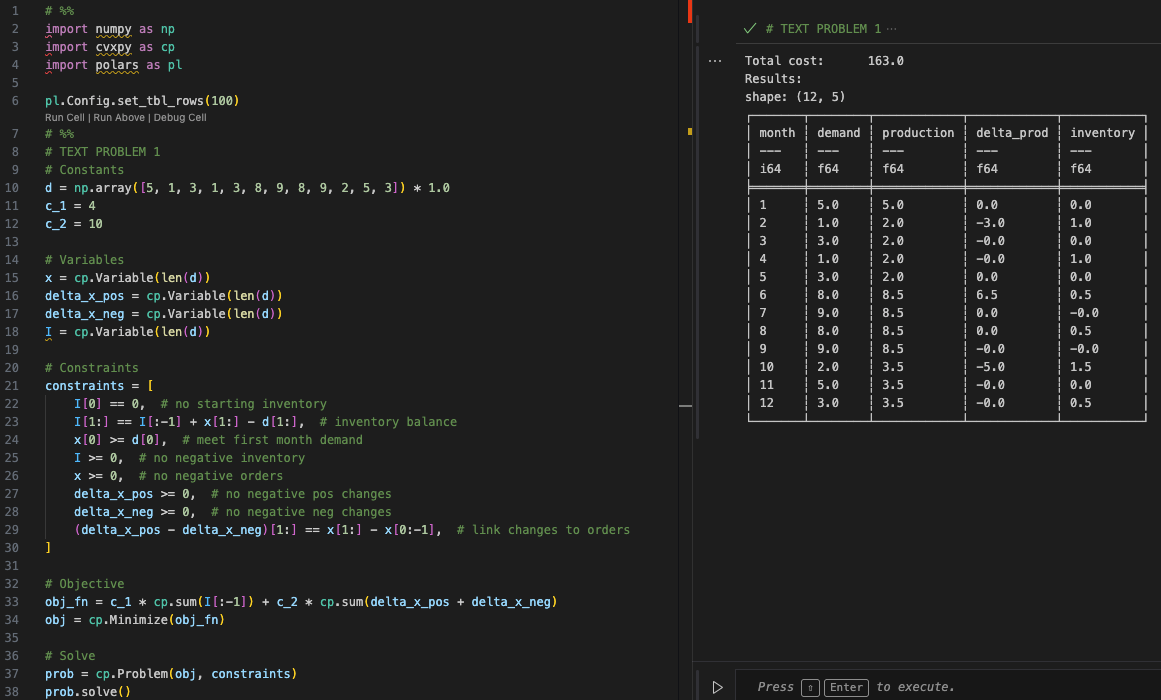
\includegraphics[width=0.9\textwidth]{problem1.png}
    \end{center}

    \question \textbf{1.7 Moment problem}
    
    Given: $Z \sim \mathcal{D}$ with $z \in \{0, 1, \dots, K\},\; p(Z=z) = p_z, \; E[Z],\; E[Z^2]$
    \newline\newline Let $z^n = [1, 2^n, \dots, K^n]^T \in \mathbb{R}^K, \; p=[p_1, \dots, p_K]^T \in \mathbb{R}^K$ 
    
    Then $E[Z] = p^Tz, \; E[Z^2] = p^Tz^2$, and $E[Z^4] = p^Tz^4$
    \newline\newline Assume $z^n,\; K,\;E[Z],\;E[Z^2]$ are known. If $p$ is known, $E[Z^4]$ can be trivially solved for. Assuming $p$ is unknown, we can use an LP to maximize and minimize $E[Z^4]$ over $p$. These solutions provide the upper and lower bounds respectively:
    \begin{align*}
        \min_p / \max_p \quad & p^Tz^4\\
        \text{s.t.}\quad & p^Tz = E[Z]\\
        & p^Tz^2 = E[Z^2]\\
        & p \geq 0, \; \textbf{1}^Tp = 1
    \end{align*}

    \question \textbf{1.12 Chebychev center}
    \begin{align*}
        \mathcal{P} = \{x \in \mathbb{R}^n \mid a_i^Tx \leq b_i,\; i=1, \dots, m \} \tag{polyhedron}\\
        \mathcal{B} = \{x \in \mathbb{R}^n \mid ||x - y||_2 \leq r \} \tag{ball with center at $y$ and radius $r$}
    \end{align*}
    We can use an optimization problem to solve for the ball centered at $y$ with maximum radius, $r$ contained within $\mathcal{P}$, but this is not an LP:
    \begin{align*}
        \max_{x, r} \quad & r\\
        \text{s.t.}\quad & a_i^Tx \leq b_i,\; i=1, \dots, m\\\
        & ||x - y||_2 \leq r\\
        & r \geq 0
    \end{align*}
    We can substitute nonlinear constraint $||x - y||_2 \leq r$ with a requirement that every line segment from ball center, $y$, to every hyperplane, $a_i^Tx = b_i$, is less than or equal to $r$. By definition, distance, $d$, from $y$ to a point, $x_{i_0}$, on hyperplane $i$ is
    \begin{align*}
        d = \frac{a_i}{||a_i||_2}^T (x_{i_0} - y) = \frac{a_i^Tx_{i_0} - a_i^Ty}{||a_i||_2} = \frac{b_i - a_i^Ty}{||a_i||_2}
    \end{align*}
    Note on sign: distance is positive in this equation when $a_i^Ty \leq b_i$, which is directly what we want for $\mathcal{B} \subseteq \mathcal{P}$
    \newline So an LP that maximizes ball radius $r$ subject to $\mathcal{B} \subseteq \mathcal{P}$ can be formulated as
    \begin{align*}
        \max \quad & r\\
        \text{s.t.}\quad & r \leq \frac{b_i - a_i^Ty}{||a_i||_2},\; i=1, \dots, m\\
        & r \geq 0
    \end{align*}

    
    \question \textbf{2.6 Caratheodory theorem}
  
  Given: $A_1, \dots, A_n \in \mathbb{R}^m$
  \begin{parts}
    \part 
    let $\mathcal{C} = \{\sum_i^n \lambda_i A_i \mid \lambda_i \geq 0 \}$ and $A=[A_1, \dots, A_n]$
    
    \textbf{Show}: For any $x = A\lambda \in \mathcal{C}$, $\exists \lambda^*\geq 0$ with $|supp(\lambda*)| \leq m$ and $x = A\lambda^*$
    \newline\newline
    \textbf{Trivial case ($n \leq m$):} by definition we have $\lambda^* = \lambda$, since any $x \in \mathcal{C} = A\lambda$ has $|supp(\lambda)| \leq n \leq m$
    \newline\newline
    \textbf{Main case ($n > m$):} Approach is to show that an algorithm exists to construct $\lambda^*$. 
    \newline\newline Algorithm: First, choose any $x \in \mathcal{C} = A\lambda = \sum_{i=1}^n \lambda_ia_i$
    \begin{enumerate}
        \item If $|supp(\lambda)| \leq m$ then stop. We have $\lambda^* = \lambda$
        \item Take any new nonzero vector $d \in \mathcal{N}(A)$ with $supp(d) \subseteq supp(\lambda)$. 
        
        We know $d$ exists since since $supp(\lambda) > m$ and $\mathcal{R}(A) \leq m$ so the columns of $A$ that are supported by $supp(\lambda)$ are linearly dependent. 
        
        Since $Ad = 0$ by definition, we can rewrite $A\lambda = A\lambda - \alpha Ad = A(\lambda - \alpha d)$
        \item Choose $\alpha$ such that $\lambda' = \lambda - \alpha d \geq 0$. This is possible since we can let 
        \begin{align*}
            \alpha = min_i \frac{\lambda_i}{d_i}, \text{ over all } i \text{ where } d_i > 0
        \end{align*}
        If $d \leq 0$, we can define new $d := -d$. Now by construction, we have zeroed out index $i_{min}$ since $\lambda'_{i_{min}} = \lambda_{i_{min}} - \frac{\lambda_{i_{min}}}{d_{i_{min}}}d_{i_{min}} = 0$. Feasibility check on the remaining indices: 
        \begin{itemize}
            \item $d_i > 0$: $\lambda'_j = \lambda_j - \frac{\lambda_{i_{min}}}{d_{i_{min}}} * d_j \Longrightarrow \frac{\lambda'_j}{d_j} = \frac{\lambda_j}{d_j} - \frac{\lambda_{i_{min}}}{d_{i_{min}}} \geq 0$ since $\frac{\lambda_j}{d_j} \geq \frac{\lambda_{i_{min}}}{d_{i_{min}}}$
            \item $d_i = 0$: $\lambda'_i = \lambda_i - \alpha 0 = \lambda_i \geq 0$
            \item $d_i < 0$: $\lambda'_i \geq \lambda_i \geq 0$ since $\alpha \geq 0$
        \end{itemize}
        \item Now we have constructed $\lambda'$ with $|supp(\lambda')| < |supp(\lambda)|$. Return to step 1 and use $\lambda'$ as $\lambda$
    \end{enumerate} 

    \part let $\mathcal{P} =\{A\lambda \mid \lambda \geq 0, \mathbf{1}^T\lambda = 1 \}$
    
    \textbf{Show:} For any $x = A\lambda \in \mathcal{P}$, $\exists \lambda^*\geq 0$ with $\mathbf{1}^T\lambda^* = 1$, $|supp(\lambda^*)| \leq m+1$, and $x = A\lambda^*$
    \newline\newline
    \textbf{Trivial case ($n < m$):} by definition we have $\lambda^* = \lambda$, since any $x \in \mathcal{P} = A\lambda$ has $|supp(\lambda)| \leq n < m < m + 1$
    \newline\newline
    \textbf{Main case ($n \geq m$):} The approach is to reframe the constraints in set $\mathcal{P}$ so that we can call on part (a). By definition, for any $x \in \mathcal{P}$, we have the following system of equations: 
    \begin{align*}
        \begin{bmatrix} A \\ \mathbf{1}^T \end{bmatrix} \lambda = \begin{bmatrix} x \\ 1\end{bmatrix}
    \end{align*} 
    We can define $\hat{A} := \begin{bmatrix} A \\ \mathbf{1}^T\end{bmatrix}\in \mathbb{R}^{m+1\times n}$ and repeat the algorithm in part (a) using $\hat{A}$ in place of $A$ and $\mathcal{R}(A) \leq m + 1$. 
    \newline\newline This demonstrates that we can construct $\lambda^*$ with $|supp(\lambda^*)| \leq m + 1$. And we know $\hat{A} \lambda^* = \begin{bmatrix} A \\ \mathbf{1}^T \end{bmatrix} \lambda^* = \begin{bmatrix} x \\ 1\end{bmatrix}$ and $\lambda^* \geq 0$ by construction.
  \end{parts}

  \question \textbf{2.13 Basic feasible solution}
  \newline \textbf{Given}: Standard form polyhedron $\mathcal{P}=\{x \mid Ax = b, x \geq 0\}$, $A \in \mathbb{R}^{m\times n}$ has $m$ linearly independent rows, and all basic feasible solutions are nondegenerate. 

  Let $x \in \mathcal{P}$ with exactly $m$ positive components
  \begin{parts}
      \part \textbf{Show:} $x$ is basic feasible solution

      Let $I = \{i \mid x_i \neq 0\}$ and $N = I^C$.
      \newline\newline \textbf{Contradiction:} Suppose $x$ is not a basic feasible solution. Since $x$ is not a BFS, but has $m$ nonzero values, then the only way it fails BT Theorem 2.4 is that the columns of $A_I = [A_i \text{ for } i \in I] \in \mathbb{R}^{m\times m}$ are linearly dependent (if they were independent, there would be a unique solution to $A_Ix_I = b$ and x would be a BFS). 
      \newline\newline Then there exists a nonzero $d_I \in \mathbb{R}^{m}$ such that $A_Id_I = 0$. For $x\in \mathcal{P}$, let $y = x - \alpha d$. If we choose $\alpha = \min_{i \in I | d_i > 0} x_i / d_i$ we have that
      \begin{itemize}
          \item $x_i - \alpha d_i \geq 0 \quad \forall i\in I \Rightarrow y_I \geq 0$
          \item $A_Iy_I = A_I(x_I - \alpha d_I) = A_Ix_I - \alpha A_Id_I = A_Ix_I + 0 = b$
          \item $y_{i_{min}} = x_{i_{min}} - \frac{x_{i_{min}}}{d_{i_{min}}}d_{i_{min}} = 0$
      \end{itemize}
      And hence $|supp(y_I)| < m$. Note, for the remaining $j \in N$, we can trivially set $d_j = 0 \Rightarrow y_j = 0$ and see that $y \in \mathcal{P}$ and hence $|supp(y)| < m$. 
      \newline\newline We may continue this dimension elimination process until we have produced $y^*$ with $|supp(y^*)| = l < m$ and linearly independent columns $A_l$ for $l \in L := \{l | y^*_l \neq 0\}$. We have constructed a BFS, $y^*$, with $l<m$ positive components, which by definition is a degenerate BFS and contradicts the given that all basic feasible solutions are nondegenerate.

    \part \textbf{Show:} The result in part (a) fails if the nondegeneracy assumption is removed. 
    \newline\newline This follows directly from our proof in part (a), where we can no longer build a contradiction to the given assumption that all basic feasible solutions are nondegenerate. To emphasize this point, I provide a counterexample. Let
    \begin{align*}
       \text{Let } &  A = \begin{bmatrix}
            1 & 1 & 0 \\
            0 & 0 & 1
        \end{bmatrix} \in \mathbb{R}^{2 \times 3} \text{ and } b = [2, 0]^T
    \end{align*}
    Defining standard form $\mathcal{P} = \{x \in \mathbb{R}^3 \mid Ax = b, x \geq 0\}$, we can choose $x = [1, 1, 0]^T \in \mathcal{P}$ and we have set up an example of the stated problem:
    \begin{itemize}
        \item $A$ has $m=2$ linearly independent rows
        \item $x$ has exactly $m=2$ positive components
    \end{itemize}
    Letting $I = \{i \mid x_i \neq 0\}$, we have $A_I = \begin{bmatrix}1 & 1 \\ 0 & 0 \end{bmatrix}$, which does not have linearly independent columns and hence $A_Ix_I = b$ does not have a unique solution and hence $x$ is not a basic feasible solution.
  \end{parts}

\end{questions}

\end{document}
